% LNCS format report for Eco-Adaptive Home Storage project
\documentclass[runningheads]{llncs}

\usepackage[T1]{fontenc}
\usepackage{graphicx}
\usepackage{amsmath}
\usepackage{amssymb}
\usepackage{booktabs}
\usepackage{multirow}
\usepackage[hidelinks]{hyperref}

\begin{document}

\title{Eco-Adaptive Home Storage: Multi-Objective Reinforcement Learning for Smart Grid Energy Management}

\titlerunning{Multi-Objective RL for Smart Grid Energy Management}

\author{Adam Younsi \and Ilyas Madah \and Zaid El Kasemy}

\authorrunning{A. Younsi, I. Madah, Z. El Kasemy}

\institute{Reinforcement Learning Course Project\\
\email{\{adam.younsi, ilyas.madah, zaid.elkasemy\}@student.edu}}

\maketitle

\begin{abstract}
We present a comparative study of reinforcement learning approaches for intelligent home battery management in smart grid environments. Our system optimizes a multi-objective reward function balancing electricity costs, carbon emissions, and battery wear. We implement and evaluate two learned agents---Deep Q-Network (DQN) with neural network function approximation and SARSA with tile coding---against multiple rule-based baselines. Through systematic hyperparameter ablation and statistical evaluation with 95\% confidence intervals, we demonstrate that SARSA with optimized tile coding achieves the best performance, with mean daily savings of \euro{}2.19 and 3.34~kg CO$_2$ avoided, outperforming both DQN and expert-designed heuristics. Our results highlight that linear function approximation with appropriate feature engineering can compete with deep learning approaches in structured domains.

\keywords{Reinforcement Learning \and Smart Grid \and Battery Management \and DQN \and SARSA \and Tile Coding \and Multi-Objective Optimization}
\end{abstract}

%==============================================================================
\section{Introduction}
%==============================================================================

Residential battery storage systems, coupled with rooftop solar generation and time-varying electricity pricing, create a complex sequential decision-making problem: when should a home battery charge, discharge, or remain idle to minimize both electricity costs and carbon emissions? Reinforcement learning (RL) is well-suited to this task, as agents can learn optimal policies through environment interaction without explicit models of price dynamics or consumption patterns~\cite{vazquez2019rl,wang2020deep}.

We formulate this problem as a Markov Decision Process (MDP) with a multi-objective reward balancing cost, emissions, and battery wear, and compare two learned agents---Deep Q-Network (DQN)~\cite{mnih2015dqn} and SARSA with tile coding~\cite{sutton2018rl}---against rule-based baselines. Our contributions include: (1) a multi-objective reward formulation; (2) systematic hyperparameter ablation for both agents; (3) statistical evaluation with confidence intervals; and (4) the finding that SARSA with tile coding outperforms DQN in this structured domain.

%==============================================================================
\section{Methods}
%==============================================================================

\subsection{Environment Formulation}

We model the smart grid battery management problem as an MDP. The RL agent acts as a \emph{battery controller}, deciding at each time step whether to charge, discharge, or leave the battery idle. The agent does not control solar production or household consumption---these are determined by the environment.

\textbf{State Space} $\mathcal{S} \subset \mathbb{R}^5$: The state vector is:
\begin{equation}
    s_t = [\text{hour}_t, \text{SoC}_t, P_{\text{net},t}, c_{\text{grid},t}, I_{\text{CO}_2,t}]
\end{equation}
where $\text{hour}_t \in [0, 24]$ is the time of day, $\text{SoC}_t \in [0, 1]$ is the battery state of charge, $P_{\text{net},t}$ is the net load (consumption minus solar production, positive indicating a deficit), $c_{\text{grid},t}$ is the electricity price (\euro{}/kWh), and $I_{\text{CO}_2,t}$ is the grid carbon intensity (gCO$_2$/kWh).

\textbf{Action Space} $\mathcal{A} = \{0, 1, 2\}$: charge (0), discharge (1), or idle (2).

\textbf{Reward Function}: We define a multi-objective reward:
\begin{equation}
    R_t = -(\alpha \cdot \text{Cost}_t + \beta \cdot \text{Emissions}_t + \gamma \cdot |a_t - a_{t-1}|)
\end{equation}
where $\alpha = 1.0$, $\beta = 0.6$, and $\gamma = 0.05$ weight the electricity cost, carbon emissions, and action switching penalty respectively. The cost and emissions at each step are computed from the grid import power: $P_{\text{grid}} = \max(P_{\text{net}} + P_{\text{batt}}, 0)$, where $P_{\text{batt}}$ is positive during charging and negative during discharging.

\textbf{Battery Dynamics}: We simulate a 10~kWh battery with 3~kW maximum power and 95\% charge/discharge efficiency. Episodes span 24 hours with 30-minute time steps (48 steps per episode).

\textbf{Synthetic Data Generation}: The environment generates realistic daily profiles for each episode. Solar production follows a bell curve centered at midday with a randomly varying peak capacity (2.5--4.0~kW). Household consumption combines a 1.4~kW base load with Gaussian-shaped morning (7:30) and evening (19:00) demand peaks, plus random noise. Electricity prices follow time-of-use patterns with an evening premium (range 0.08--0.45~\euro{}/kWh), and carbon intensity is higher during evening peak hours when fossil fuel plants ramp up (range 150--700~gCO$_2$/kWh). Random variation in all profiles ensures each episode represents a unique day.

\subsection{Deep Q-Network (DQN)}

DQN approximates the action-value function using a neural network $Q(s, a; \theta)$ with experience replay and a target network for stability~\cite{mnih2015dqn}. The loss function is:
\begin{equation}
    \mathcal{L}(\theta) = \mathbb{E}_{(s,a,r,s') \sim \mathcal{D}} \left[ \left( r + \gamma \max_{a'} Q(s', a'; \theta^-) - Q(s, a; \theta) \right)^2 \right]
\end{equation}
We conduct an ablation study over three network architectures: Small [32, 32], Medium [64, 64], and Large [128, 64] hidden layers, all with layer normalization.

\subsection{SARSA with Tile Coding}

SARSA is an on-policy TD control algorithm with update rule:
\begin{equation}
    Q(S_t, A_t) \leftarrow Q(S_t, A_t) + \alpha \left[ R_{t+1} + \gamma Q(S_{t+1}, A_{t+1}) - Q(S_t, A_t) \right]
\end{equation}
For function approximation, we use tile coding~\cite{sutton2018rl}, which creates sparse binary feature vectors through multiple overlapping tilings. The value function is linear: $Q(s, a) = \mathbf{w}_a^\top \phi(s)$, where $\phi(s)$ is the tile coding feature vector. We use 32 tilings with 4 tiles per dimension, providing fine resolution with minimal aliasing.

\subsection{Baseline Agents}

We compare against five baselines: \textbf{Greedy} (charges below 0.15~\euro{}/kWh, discharges above 0.28), \textbf{EcoGreedy} (threshold-based on carbon intensity), \textbf{Threshold} (time-scheduled: charge hours 0--6, discharge 17--21), \textbf{Random} (uniform action selection), and \textbf{Idle} (no battery usage, serves as savings reference).

%==============================================================================
\section{Experimental Setup}
%==============================================================================

\textbf{Training}: DQN agents are trained for 2,000 episodes per configuration with $\epsilon$-greedy exploration ($\epsilon$: $1.0 \rightarrow 0.05$, decay 0.995). SARSA agents are trained for 3,000 episodes with slower decay ($\epsilon$: $1.0 \rightarrow 0.02$, decay 0.998) to allow more thorough exploration.

\textbf{Evaluation}: All agents are evaluated over 100 episodes with fixed random seeds. We report mean performance with 95\% confidence intervals computed using the t-distribution.

\textbf{Metrics}: We measure (1) cumulative reward, (2) daily electricity savings vs.\ idle baseline (\euro{}), and (3) CO$_2$ emissions avoided vs.\ baseline (kg).

\textbf{Implementation}: Code follows the RL-GLUE framework~\cite{tanner2009rlglue}. DQN uses PyTorch; SARSA requires only NumPy.

%==============================================================================
\section{Results and Discussion}
%==============================================================================

\subsection{Hyperparameter Ablation}

Table~\ref{tab:ablation} presents the ablation results for both agents. For DQN, the Medium architecture [64, 64] achieves the best performance, suggesting larger networks may overfit to the relatively low-dimensional state space. For SARSA, standard SARSA slightly outperforms Expected SARSA, which uses the expected value under the policy rather than the sampled next action.

\begin{table}[t]
\caption{Ablation study results. DQN trained 2,000 episodes; SARSA trained 3,000 episodes with 32 tilings $\times$ 4 tiles.}\label{tab:ablation}
\centering
\begin{tabular}{llcc}
\toprule
\textbf{Agent} & \textbf{Configuration} & \textbf{Mean Reward} & \textbf{Time (s)} \\
\midrule
DQN-Small & [32, 32] & $-13.68$ & 532 \\
DQN-Medium & [64, 64] & $\mathbf{-13.26}$ & 510 \\
DQN-Large & [128, 64] & $-14.61$ & 518 \\
\midrule
SARSA & Standard & $\mathbf{-10.98}$ & 75 \\
Expected SARSA & Standard & $-11.24$ & 79 \\
\bottomrule
\end{tabular}
\end{table}

\subsection{Final Agent Comparison}

Table~\ref{tab:comparison} presents the comprehensive evaluation results. SARSA achieves the best overall performance across all metrics, with statistically significant improvements over DQN. Both learned agents outperform all rule-based baselines.

\begin{table}[t]
\caption{Agent comparison with 95\% confidence intervals (100 evaluation episodes).}\label{tab:comparison}
\centering
\begin{tabular}{llccc}
\toprule
\textbf{Agent} & \textbf{Type} & \textbf{Reward} & \textbf{Savings (\euro{})} & \textbf{CO$_2$ Avoided (kg)} \\
\midrule
SARSA & Learned & $\mathbf{-10.88 \pm 0.79}$ & $\mathbf{2.194 \pm 0.267}$ & $\mathbf{3.336 \pm 0.411}$ \\
DQN & Learned & $-12.93 \pm 1.68$ & $1.131 \pm 0.708$ & $1.888 \pm 1.099$ \\
Threshold & Rule-based & $-12.98 \pm 0.72$ & $1.274 \pm 0.366$ & $1.450 \pm 0.627$ \\
EcoGreedy & Rule-based & $-14.16 \pm 0.88$ & $0.760 \pm 0.477$ & $0.543 \pm 0.759$ \\
Greedy & Rule-based & $-14.48 \pm 0.85$ & $0.551 \pm 0.480$ & $0.448 \pm 0.698$ \\
Idle & Baseline & $-14.82 \pm 0.51$ & $0.000 \pm 0.000$ & $0.000 \pm 0.000$ \\
Random & Baseline & $-21.91 \pm 1.88$ & $-2.427 \pm 0.892$ & $-4.175 \pm 1.478$ \\
\bottomrule
\end{tabular}
\end{table}

\begin{figure}[t]
\centering
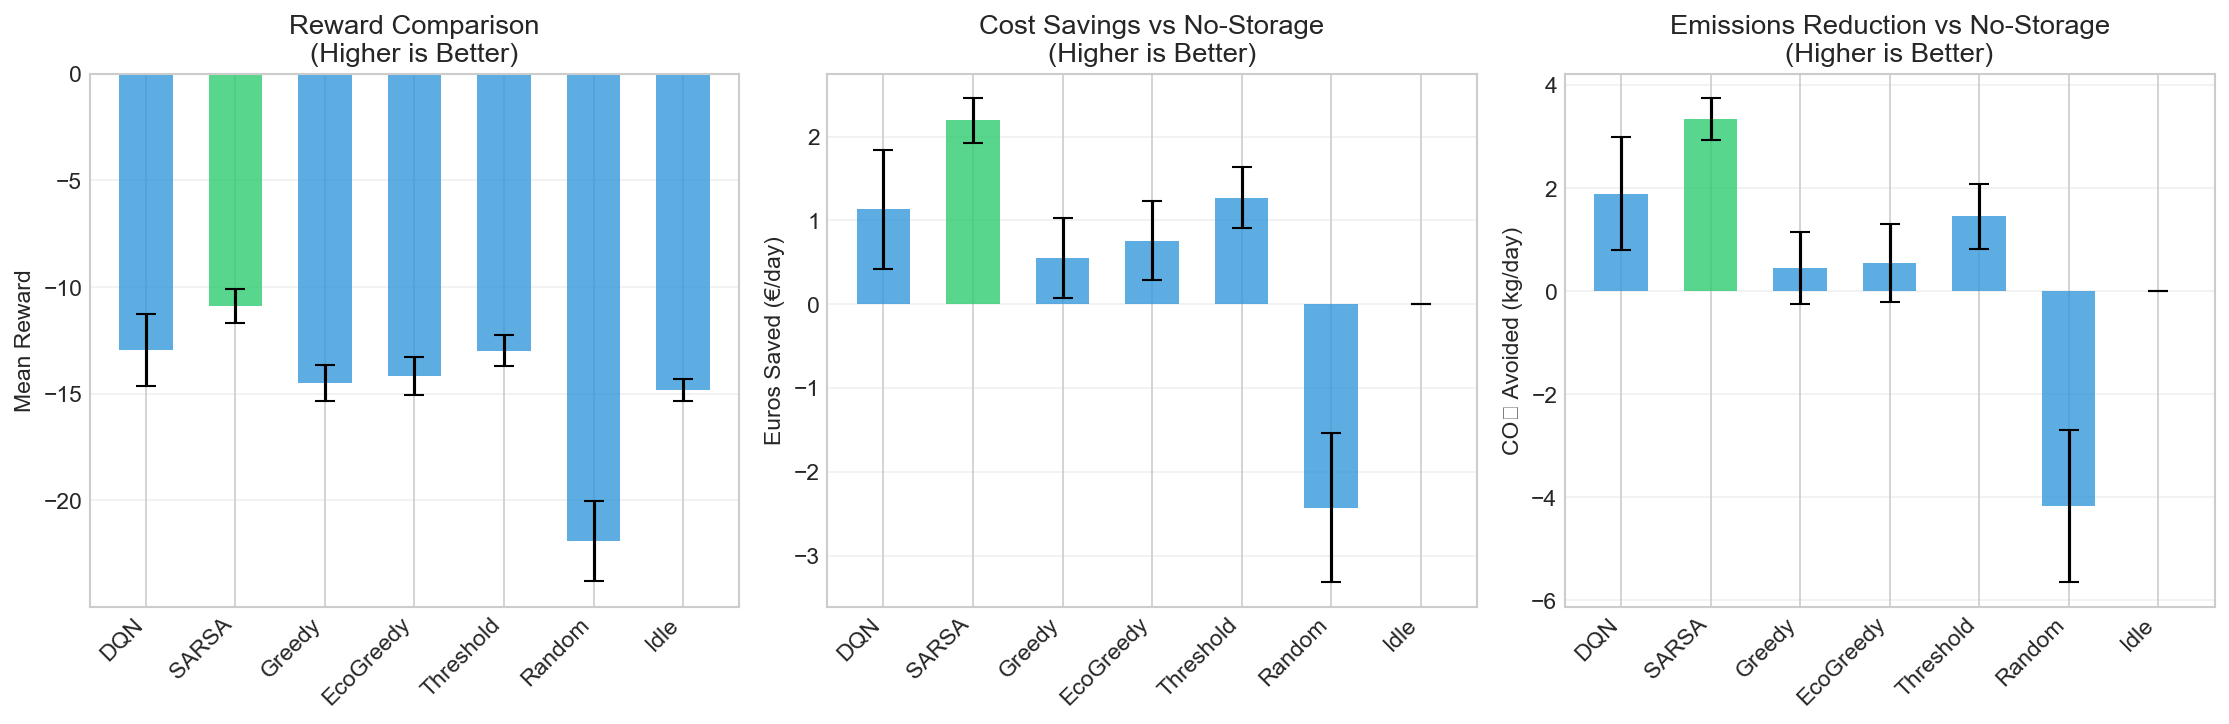
\includegraphics[width=0.95\textwidth]{figures/agent_comparison.png}
\caption{Agent comparison with error bars: (Left) Mean reward, (Center) Daily savings, (Right) CO$_2$ avoided. Higher values are better for all metrics.}\label{fig:comparison}
\end{figure}

\subsection{Discussion}

\textbf{SARSA outperforms DQN}: SARSA with tile coding achieves 15.9\% better reward than the best DQN configuration ($-10.88$ vs.\ $-12.93$), with notably tighter confidence intervals ($\pm 0.79$ vs.\ $\pm 1.68$), indicating a more stable policy. We attribute this to the structured nature of the 5-dimensional state space, where tile coding provides appropriate inductive bias for local generalization. Additionally, SARSA benefits from greater training stability and more thorough exploration through slower $\epsilon$ decay over more episodes.

\textbf{Threshold baseline is competitive}: The Threshold agent achieves reward comparable to DQN ($-12.98$ vs.\ $-12.93$), confirming that domain knowledge---charge at night, discharge in the evening---captures significant value. However, learned agents adapt better to daily variability in prices and solar production.

\textbf{Computational efficiency}: SARSA trains in $\sim$75s vs.\ $\sim$510s for DQN (7$\times$ speedup), requiring no GPU or deep learning framework, while achieving superior performance.

%==============================================================================
\section{Conclusion}
%==============================================================================

We presented a comparative study of reinforcement learning for smart grid battery management. Our multi-objective formulation balances electricity cost, carbon emissions, and battery wear. Through systematic evaluation, we demonstrated that:

\begin{enumerate}
    \item SARSA with tile coding achieves the best performance (\euro{}2.19 daily savings, 3.34~kg CO$_2$ avoided), outperforming DQN by 15.9\% in mean reward.
    \item Medium-sized DQN architectures [64, 64] outperform both smaller and larger networks.
    \item Linear function approximation with appropriate features can compete with deep learning in structured domains.
    \item The Threshold heuristic provides a strong baseline, highlighting the value of domain knowledge.
\end{enumerate}

Future work includes extending to continuous action spaces, incorporating real-world price data, and exploring model-based approaches for improved sample efficiency.

\begin{credits}
\subsubsection{\ackname} This work was completed as part of the Reinforcement Learning course. We thank the course instructors for guidance on the RL-GLUE framework and evaluation methodology.
\end{credits}

\begin{thebibliography}{8}

\bibitem{mnih2015dqn}
Mnih, V., et al.: Human-level control through deep reinforcement learning. Nature \textbf{518}(7540), 529--533 (2015)

\bibitem{sutton2018rl}
Sutton, R.S., Barto, A.G.: Reinforcement Learning: An Introduction. 2nd edn. MIT Press, Cambridge (2018)

\bibitem{tanner2009rlglue}
Tanner, B., White, A.: RL-Glue: Language-independent software for reinforcement-learning experiments. Journal of Machine Learning Research \textbf{10}, 2133--2136 (2009)

\bibitem{vazquez2019rl}
V\'{a}zquez-Canteli, J.R., Nagy, Z.: Reinforcement learning for demand response: A review of algorithms and modeling techniques. Applied Energy \textbf{235}, 1072--1089 (2019)

\bibitem{rocchetta2019battery}
Rocchetta, R., Bellani, L., Compare, M., Zio, E., Patelli, E.: A reinforcement learning framework for optimal operation of a battery in presence of renewable energy sources. Renewable Energy \textbf{139}, 504--515 (2019)

\bibitem{wang2020deep}
Wang, J., et al.: Deep reinforcement learning for energy management in smart grids: A survey. IEEE Transactions on Industrial Informatics \textbf{16}(12), 7734--7744 (2020)

\end{thebibliography}

\end{document}
